\documentclass[border=12pt]{standalone}
\def\pgfsysdriver{pgfsys-dvisvgm.def}
\usepackage[dvisvgm]{xcolor}
\usepackage{xeCJK}
\setCJKmainfont{HaranoAjiGothic-Regular.otf}[BoldFont=HaranoAjiGothic-Bold.otf]
\setCJKsansfont{HaranoAjiGothic-Regular.otf}[BoldFont=HaranoAjiGothic-Bold.otf]
\usepackage{amsmath,amssymb,tikz,lmodern}
\usetikzlibrary{arrows.meta,positioning,calc,fit,backgrounds}
\renewcommand{\familydefault}{\sfdefault}
\definecolor{ink}{HTML}{25322F}
\definecolor{green}{HTML}{246657}
\definecolor{tint}{HTML}{EEF4F0}
\definecolor{soft}{HTML}{C6D2CC}
\definecolor{muted}{HTML}{52615B}
\newif\ifJapanese
\newcommand{\Tx}[2]{\ifJapanese #1\else #2\fi}
\newcommand{\Eff}{\overline{\operatorname{Eff}}}
\newcommand{\heading}[3]{{\color{green}\bfseries #1\quad\Tx{#2}{#3}}\\[5pt]}
% A white rectangle makes the complete citation label clickable, including spaces.
\newcommand{\refurl}[2]{\special{dvisvgm:raw <a xlink:href="#1" target="_blank" rel="noopener noreferrer">}{\setlength{\fboxsep}{0pt}\colorbox{white}{\color{green}\underline{\strut #2}}}\special{dvisvgm:raw </a>}}
\newcommand{\refedge}[3]{\refurl{\csname source#1\endcsname\string##page=#2}{#3}}
\newcommand{\SF}[2]{\refedge{sf}{#1}{#2}}
% GitHub's file preview does not support PDF page fragments.
\newcommand{\LA}[2]{\refurl{\sourcela}{#2}}
\newcommand{\Sch}[2]{\refedge{sch}{#1}{#2}}
\newcommand{\PS}[2]{\refedge{ps}{#1}{#2}}
\tikzset{
 card/.style={draw=soft,fill=white,rounded corners=2pt,align=left,text=ink,font=\fontsize{10.5}{14}\selectfont,inner xsep=12pt,inner ysep=10pt,text width=14.4cm},
 half/.style={card,text width=6.45cm,minimum height=2.05cm},
 result/.style={card,draw=green,fill=tint,line width=.9pt},
 reason/.style={align=left,text=muted,font=\fontsize{9}{12}\selectfont,inner sep=0pt,text width=12.7cm},
 branchreason/.style={reason,text width=5.95cm},
 edge/.style={-{Stealth[length=2.4mm]},draw=green,line width=1pt},
 wire/.style={draw=green,line width=1pt},
}
% Keep the arrow in a dedicated left gutter; explanations never cover it.
\newcommand{\flow}[3]{
 \coordinate (#2-from) at ($(#1.south)+(-6.9,0)$);
 \coordinate (#2-to) at ($(#2.north)+(-6.9,0)$);
 \draw[edge] (#2-from)--(#2-to);
 \node[reason,anchor=west] (#2-reason) at ($(#2-from)!.5!(#2-to)+(.55,0)$) {#3};
}


\newcommand{\CiteSource}[2]{\refurl{\csname source#1\endcsname}{#2}}

\expandafter\def\csname sourceRD\endcsname{https://github.com/openai/math/blob/adc7f1241b42e322a6451854ab7e4b4c146bf78a/preprints/Relative-denominators-and-effective-systems-for-log-Calabi-Yau-fibrations-September-27-2026/paper.pdf}
\expandafter\def\csname sourceSL\endcsname{https://github.com/openai/math/blob/adc7f1241b42e322a6451854ab7e4b4c146bf78a/preprints/Lifting-sections-from-the-reduced-support-of-an-adjoint-September-27-2026/paper.pdf}
\expandafter\def\csname sourceLA\endcsname{https://github.com/openai/math/blob/adc7f1241b42e322a6451854ab7e4b4c146bf78a/preprints/Log-abundance-in-characteristic-zero-September-24-2026/paper.pdf}
\expandafter\def\csname sourceJL\endcsname{https://arxiv.org/pdf/2002.11928v1}
\expandafter\def\csname sourceXu\endcsname{https://arxiv.org/pdf/1905.00297v2}
\expandafter\def\csname sourceCT\endcsname{https://arxiv.org/pdf/2011.02236v2}
\expandafter\def\csname sourceUfour\endcsname{https://github.com/openai/math/blob/adc7f1241b42e322a6451854ab7e4b4c146bf78a/preprints/Uniform-effective-log-Iitaka-fibrations-for-fourfolds-September-26-2026/paper.pdf}

\Japanesefalse
\begin{document}
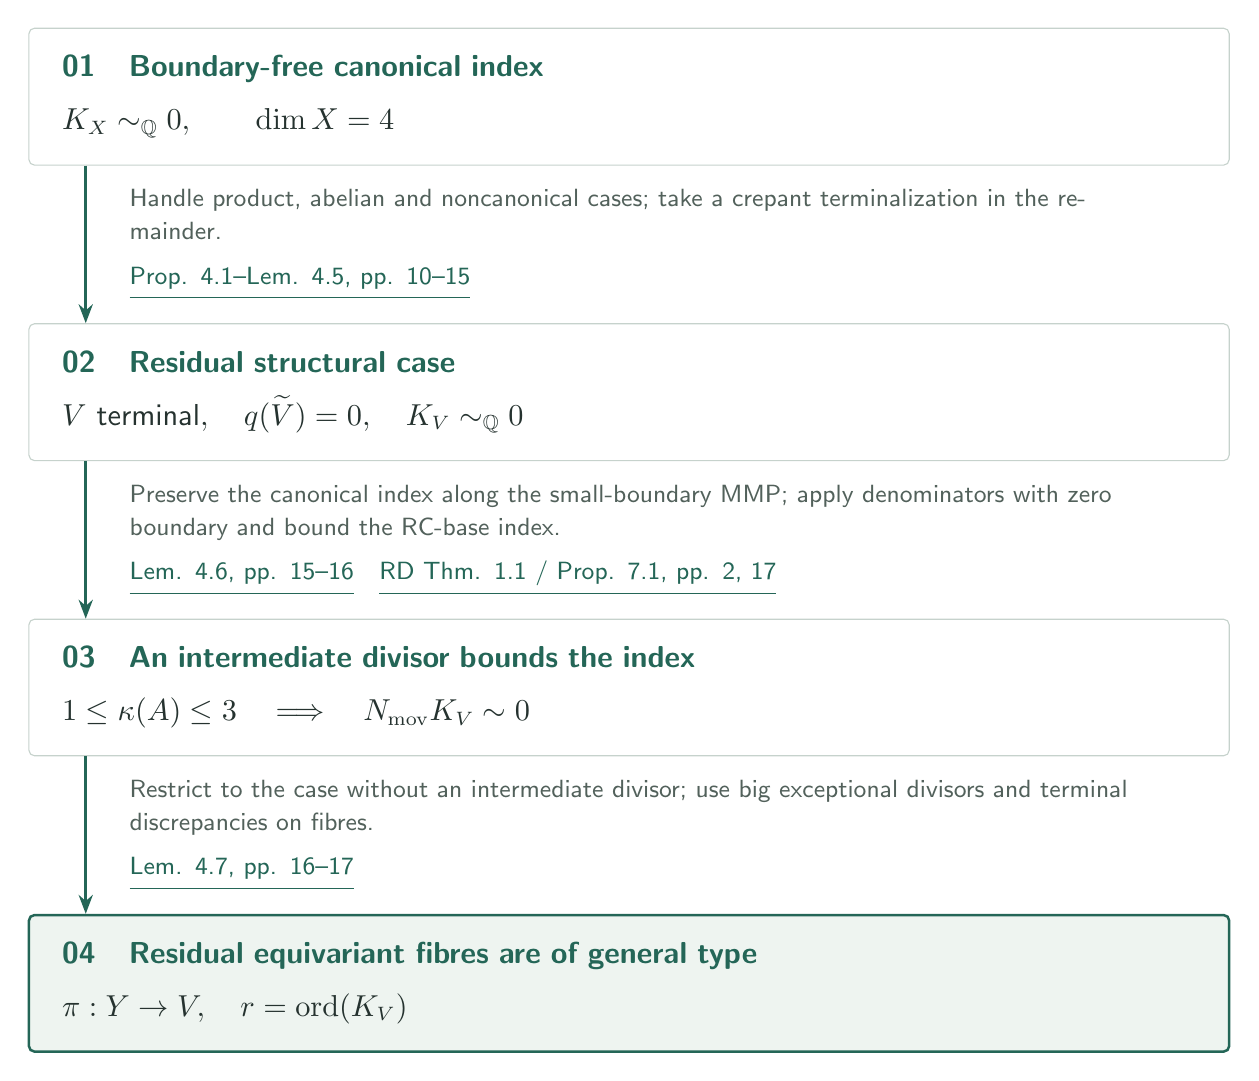
\begin{tikzpicture}
\node[card] (n0) {\heading{01}{境界なし標準指数}{Boundary-free canonical index}$K_X\sim_{\mathbb Q}0,\qquad \dim X=4$};
\node[card,below=2.0cm of n0] (n1) {\heading{02}{構造で分離した残余の場合}{Residual structural case}$V\text{ terminal},\quad q(\widetilde V)=0,\quad K_V\sim_{\mathbb Q}0$};
\flow{n0}{n1}{\Tx{積・アーベルの場合と非canonicalの場合を処理。残りをcrepantにterminal化する。}{Handle product, abelian and noncanonical cases; take a crepant terminalization in the remainder.}\\[4pt]\CiteSource{Ufour}{Prop. 4.1--Lem. 4.5, pp. 10--15}}
\node[card,below=2.0cm of n1] (n2) {\heading{03}{中間因子があれば指数を制御}{An intermediate divisor bounds the index}$1\leq\kappa(A)\leq3\quad\Longrightarrow\quad N_{\mathrm{mov}}K_V\sim0$};
\flow{n1}{n2}{\Tx{小さい境界のMMPで標準指数を保ち、境界ゼロで相対分母を適用。RCな底の指数を抑える。}{Preserve the canonical index along the small-boundary MMP; apply denominators with zero boundary and bound the RC-base index.}\\[4pt]\CiteSource{Ufour}{Lem. 4.6, pp. 15--16}\quad \CiteSource{RD}{RD Thm. 1.1 / Prop. 7.1, pp. 2, 17}}
\node[result,below=2.0cm of n2] (n3) {\heading{04}{残余の同変ファイバーは一般型}{Residual equivariant fibres are of general type}$\pi:Y\to V,\quad r=\operatorname{ord}(K_V)$};
\flow{n2}{n3}{\Tx{中間因子のない場合に限定。例外因子のbignessとterminal discrepancyをファイバー上へ制限する。}{Restrict to the case without an intermediate divisor; use big exceptional divisors and terminal discrepancies on fibres.}\\[4pt]\CiteSource{Ufour}{Lem. 4.7, pp. 16--17}}
\end{tikzpicture}
\end{document}
